%                                                                 aa.tex
% AA vers. 9.2, LaTeX class for Astronomy & Astrophysics
% Demonstration file
%                                                       (c) EDP Sciences
%-----------------------------------------------------------------------
%
%\documentclass[referee]{aa}    % for a referee version
%\documentclass[onecolumn]{aa}  % for a paper on 1 column  
%\documentclass[longauth]{aa}   % for the long lists of affiliations
%\documentclass[letter]{aa}     % for the letters
%\documentclass[bibyear]{aa}    % if the references are not structured
                                % according to the author-year natbib style

\documentclass{aa}  

\usepackage{graphicx}
\usepackage{txfonts}
\usepackage{lipsum}
\usepackage{subcaption}         % necessary for continued figures, example in section 3
                                % and appendix
\usepackage{lscape}             % to rotate a single page table, example in appendix.
                                % For landscape tables, see the longtable examples.
\usepackage{placeins}           % useful with \FloatBarrier, to keep 
                                % onecolumn floats from drifting to the next section
                                
%%%%%%%%%%%%%%%%%%%%%%%%%%%%%%%%%%%%%%%%
%\usepackage[options]{hyperref}
% To add links in your PDF file, use the package "hyperref"
% with options according to your LaTeX or PDFLaTeX drivers.
%%%%%%%%%%%%%%%%%%%%%%%%%%%%%%%%%%%%%%%%

\begin{document}

   \title{Astronomy \& Astrophysics \LaTeX\ template}

   \subtitle{Subtitle}

   \author{N. Puyaubreau\inst{1}
        \and F. Déliat\inst{2}\fnmsep\thanks{Shows the usage of elements in the author field}
        }

   \institute{EDP Sciences, 91940, Les Ulis, France\\
             \email{nicolas.puyaubreau@edpsciences.org}
             \thanks{Shows the usage of elements in the author field}
            \and EDP Sciences, 91940, Les Ulis, France\\ }

   \date{Received September 30, 20XX}

% \abstract{}{}{}{}{}
% 5 {} token are mandatory
 
  \abstract
  % context heading (optional)
  % {} leave it empty if necessary  
   {Optional, leave empty if necessary.  The heading “Context” is used when needed to
give background information on the research conducted in the paper}
  % aims heading (mandatory)
   {Mandatory. The objectives of the paper are defined here.} 
  % methods heading (mandatory)
   {Mandatory. The methods of the investigation are outlined here}
  % results heading (mandatory)
   {Mandatory. The results are summarized here.}
  % conclusions heading (optional), leave it empty if necessary
   {Optional, leave empty if necessary.  “Conclusions” can be used to
explicit the general conclusions that can be drawn from the paper.}

   \keywords{giant planet formation --
                $\kappa$-mechanism --
                stability of gas spheres
               }

   \maketitle


%%%%%%%%%%%%%%%%%%%%%%%%%%%%%%%%%%%%%%%%%%%%%%%%%%%%%%%%%%%%%%
\section{Introduction}
\lipsum[1]
%%%%%%%%%%%%%%%%%%%%%%%%%%%%%%%%%%%%%%%%%%%%%%%%%%%%%%%%%%%%%%
\section{Citations and maths examples}

   In this section the one-zone model of \citet{baker},
   originally used to study the Cephe{\"{\i}}d pulsation mechanism, will
   be briefly reviewed, see Fig.~\ref{fig1}, Table~\ref{t7} and Eq. (\ref{eq3}).
   For the one-zone-model Baker obtains necessary conditions
   for dynamical, secular and vibrational (or pulsational)
   stability (Eqs.\ (34a,\,b,\,c) in Baker \citeyear{baker}).
   
   \begin{equation}
    \label{eq1}
      \tau_{\mathrm{co}} = \frac{E_{\mathrm{th}}}{L_{r0}} \,,
   \end{equation}
   and the \emph{local free-fall time}
   \begin{equation}
      \tau_{\mathrm{ff}} =
         \sqrt{ \frac{3 \pi}{32 G} \frac{4\pi r_0^3}{3 M_{\mathrm{r}}}
}\,,
   \end{equation}
   Baker's $K$ and $\sigma_0$ have the following form:
   \begin{eqnarray}
   \label{eq3}
      \sigma_0 & = & \frac{\pi}{\sqrt{8}}
                     \frac{1}{ \tau_{\mathrm{ff}}} \\
      K        & = & \frac{\sqrt{32}}{\pi} \frac{1}{\delta}
                        \frac{ \tau_{\mathrm{ff}} }
                             { \tau_{\mathrm{co}} }\,;
   \end{eqnarray}
   where $ E_{\mathrm{th}} \approx m (P_0/{\rho_0})$ has been used and
   \begin{equation}
   \begin{array}{l}
      \delta = - \left(
                    \frac{ \partial \ln \rho }{ \partial \ln T }
                 \right)_P \\
      e=mc^2
   \end{array}
   \end{equation}
   is a thermodynamical quantity which is of order $1$ and equal to $1$
   for nonreacting mixtures of classical perfect gases. The physical
   meaning of $ \sigma_0 $ and $K$ is clearly visible in the equations
   above. $\sigma_0$ represents a frequency of the order one per
   free-fall time. $K$ is proportional to the ratio of the free-fall
   time and the cooling time. Substituting into Baker's criteria, using
   thermodynamic identities and definitions of thermodynamic quantities,
   \begin{displaymath}
      \Gamma_1      = \left( \frac{ \partial \ln P}{ \partial\ln \rho}
                           \right)_{S}    \, , \;
      \chi^{}_\rho  = \left( \frac{ \partial \ln P}{ \partial\ln \rho}
                           \right)_{T}    \, , \;
      \kappa^{}_{P} = \left( \frac{ \partial \ln \kappa}{ \partial\ln P}
                           \right)_{T}
   \end{displaymath}
   \begin{displaymath}
      \nabla_{\mathrm{ad}} = \left( \frac{ \partial \ln T}
                             { \partial\ln P} \right)_{S} \, , \;
      \chi^{}_T       = \left( \frac{ \partial \ln P}
                             { \partial\ln T} \right)_{\rho} \, , \;
      \kappa^{}_{T}   = \left( \frac{ \partial \ln \kappa}
                             { \partial\ln T} \right)_{T}
   \end{displaymath}



%_____________________________________________________________
%                     Onecolumn continued float (place early!)
%-------------------------------------------------------------
   \begin{figure*}
        \centering
        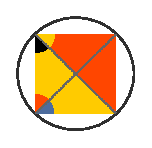
\includegraphics{figure.eps}
        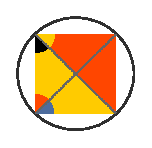
\includegraphics[angle=90]{figure.eps}
        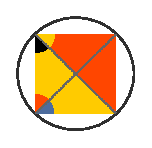
\includegraphics{figure.eps}
        {\caption{A onecolumn \textbackslash figure* with six graphics}}
        \ContinuedFloat %      \usepackage{subcaption}
        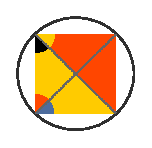
\includegraphics[angle=90]{figure.eps}
        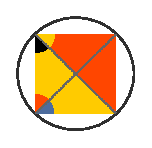
\includegraphics{figure.eps}
        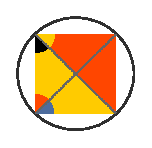
\includegraphics[angle=90]{figure.eps}
        \caption{continued.}
        \label{FigGam}%
    \end{figure*}

% %_____________________________________________________________
% %                      Another onecolumn float (place early!)
% %-------------------------------------------------------------
% \begin{figure*}[h!]
%    \resizebox{\hsize}{!}
%             {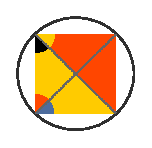
\includegraphics {figure.eps}}
%             %{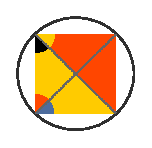
\includegraphics[bb=10 20 100 100,clip]{figure.eps}}
%       \caption{Another onecolumn figure*}
%          \label{wide}
% \end{figure*}
% \twocolumn
% \clearpage
% % %%%%%%%%%%%%%%%%%%%%%%%%%%%%%%%%%%%%%%%%%%%%%%%%%%%%%%%%%%%%%%


\section{Figures examples}
Examples of figures using graphicx. 
The guide "Using Imported Graphics in LaTeX2e" by Keith Reckdahl
is available on a lot of \LaTeX public servers or CTAN mirrors.


%_____________________________________________________________
%                        A figure as large as the column width
%-------------------------------------------------------------
   \begin{figure}[h!]
   \centering
   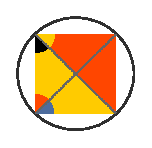
\includegraphics[width=\hsize]{figure.eps}
      \caption{Figure as large as the column width}
         \label{fig1}
   \end{figure}
%
%_____________________________________________________________
%                                             A rotated figure
%-------------------------------------------------------------
   \begin{figure}[h!]
   \centering
   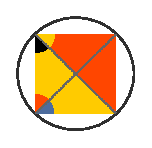
\includegraphics[angle=-90,width=2cm]{figure.eps}
      \caption{Rotated figure}
         \label{fig2}
   \end{figure}
%
%_____________________________________________________________
%                        Figure with caption on the right side
%-------------------------------------------------------------
   \begin{figure}[h!]
   \sidecaption
   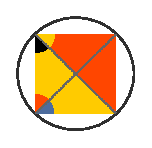
\includegraphics[width=2cm]{figure.eps}
      \caption{Figure with caption on the right side}
         \label{fig3}
   \end{figure}


%_____________________________________________________________
%                                Figure with a new BoundingBox
%-------------------------------------------------------------
   \begin{figure}
   \centering
   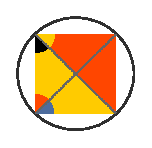
\includegraphics[bb=5 20 60 60,width=3cm,clip]{figure.eps}
      \caption{Figure with a new BoundingBox}
         \label{fig4}
   \end{figure}



%_____________________________________________________________
%                              A figure including two graphics
%-------------------------------------------------------------
   \begin{figure}[h!]
   \centering
    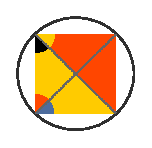
\includegraphics{figure.eps}
    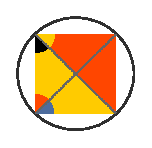
\includegraphics[angle=90]{figure.eps}
    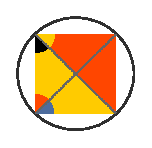
\includegraphics{figure.eps}
      \caption{A figure including three graphics}
         \label{fig5}
   \end{figure}


%_____________________________________________________________
%                                   Continued figure numbering
%      \usepackage{subcaption} and the command \ContinuedFloat
%-------------------------------------------------------------

    \begin{figure}
    \centering
    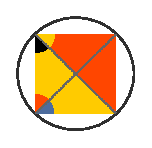
\includegraphics[width=3cm]{figure.eps}
      \caption{Continued figure numbering}
         \label{cont1}
    
    \centering
    \ContinuedFloat %      \usepackage{subcaption}
    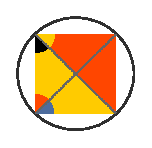
\includegraphics[width=3cm]{figure.eps}
        \caption{continued.}
             \label{cont2}

    \centering
    \ContinuedFloat %      \usepackage{subcaption}
    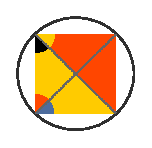
\includegraphics[width=3cm]{figure.eps}
        \caption{continued.}
             \label{cont3}
    \end{figure}


\clearpage

%%%%%%%%%%%%%%%%%%%%%%%%%%%%%%%%%%%%%%%%%%%%%%%%%%%%%%%%%%%%%%
\section{Tables examples}



The jump in table numbering below is caused by the command
\textbackslash longtable*. This command only works in the onecolumn
environment. For this reason, we recommend either:
\begin{itemize}
\item placing your long tables in onecolumn appendices (cf.~\ref{ltapp} and ~\ref{lsltapp}),
\item or using the longtab environment as illustrated by tables ~\ref{longtable1} and ~\ref{longtable2}.
Note that the longtab environment will preserve the table
numbering and automatically places long tables after the appendices.
They will be moved inside the appendices by the Publisher, if necessary.
\end{itemize}

%_____________________________________________________________
%                                             Simple A&A Table
%-------------------------------------------------------------
\begin{table}[h!]
\caption{Simple A\&A Table}                 % title of Table
\label{table:1}    % is used to refer this table in the text
\centering                        % used for centering table
\begin{tabular}{c c c c}      % centered columns (4 columns)
\hline\hline               % inserts double horizontal lines
HJD & $E$ & Method\#2 & Method\#3 \\         % table heading
\hline                      % inserts single horizontal line
   1 & 50 & $-837$ & 970 \\    % inserting body of the table
   2 & 47 & 877    & 230 \\
\hline                                  %inserts single line
\end{tabular}
\end{table}


%%%%%%%%%%%%%%%%%%%%%%%%%%%%%%%%%%%%%%%%%%%%%%%%%%%%%%%%%%%%%%%
%                                                  Long tables
%%%%%%%%%%%%%%%%%%%%%%%%%%%%%%%%%%%%%%%%%%%%%%%%%%%%%%%%%%%%%%%
%_____________________________________________________________
%                     Long table using the longtab environment
%-------------------------------------------------------------
\longtab[1]{
\begin{longtable}{lllrrr}
\caption{A long table using the longtab environment}\\
\label{longtable1}
\hline
Catalogue& $M_{V}$ & Spectral & Distance & Mode & Count Rate \\
\hline
\endfirsthead
\caption{continued.}\\
\hline\hline
Catalogue& $M_{V}$ & Spectral & Distance & Mode & Count Rate \\
\hline
\endhead
\hline
\endfoot
%%
Gl 33    & 6.37 & K2 V & 7.46 & S & 0.043170\\
Gl 66AB  & 6.26 & K2 V & 8.15 & S & 0.260478\\
Gl 68    & 5.87 & K1 V & 7.47 & P & 0.026610\\
         &      &      &      & H & 0.008686\\
Gl 86
\footnote{Source not included in the HRI catalog. See Sect.~5.4.2 for details.}
         & 5.92 & K0 V & 10.91& S & 0.058230\\
                  & 5.92 & K0 V & 10.91& S & 0.058230\\
Gl 33    & 6.37 & K2 V & 7.46 & S & 0.043170\\
Gl 66AB  & 6.26 & K2 V & 8.15 & S & 0.260478\\
Gl 68    & 5.87 & K1 V & 7.47 & P & 0.026610\\
         &      &      &      & H & 0.008686\\
Gl 86    & 5.92 & K0 V & 10.91& S & 0.058230\\            & 5.92 & K0 V & 10.91& S & 0.058230\\
Gl 33    & 6.37 & K2 V & 7.46 & S & 0.043170\\
Gl 66AB  & 6.26 & K2 V & 8.15 & S & 0.260478\\
Gl 68    & 5.87 & K1 V & 7.47 & P & 0.026610\\
         &      &      &      & H & 0.008686\\
Gl 86    & 5.92 & K0 V & 10.91& S & 0.058230\\            & 5.92 & K0 V & 10.91& S & 0.058230\\
Gl 33    & 6.37 & K2 V & 7.46 & S & 0.043170\\
Gl 66AB  & 6.26 & K2 V & 8.15 & S & 0.260478\\
Gl 68    & 5.87 & K1 V & 7.47 & P & 0.026610\\
         &      &      &      & H & 0.008686\\
Gl 86    & 5.92 & K0 V & 10.91& S & 0.058230\\            & 5.92 & K0 V & 10.91& S & 0.058230\\
Gl 33    & 6.37 & K2 V & 7.46 & S & 0.043170\\
Gl 66AB  & 6.26 & K2 V & 8.15 & S & 0.260478\\
Gl 68    & 5.87 & K1 V & 7.47 & P & 0.026610\\
         &      &      &      & H & 0.008686\\
Gl 86    & 5.92 & K0 V & 10.91& S & 0.058230\\            & 5.92 & K0 V & 10.91& S & 0.058230\\
Gl 33    & 6.37 & K2 V & 7.46 & S & 0.043170\\
Gl 66AB  & 6.26 & K2 V & 8.15 & S & 0.260478\\
Gl 68    & 5.87 & K1 V & 7.47 & P & 0.026610\\
         &      &      &      & H & 0.008686\\
Gl 86    & 5.92 & K0 V & 10.91& S & 0.058230\\            & 5.92 & K0 V & 10.91& S & 0.058230\\
Gl 33    & 6.37 & K2 V & 7.46 & S & 0.043170\\
Gl 66AB  & 6.26 & K2 V & 8.15 & S & 0.260478\\
Gl 68    & 5.87 & K1 V & 7.47 & P & 0.026610\\
         &      &      &      & H & 0.008686\\
Gl 86    & 5.92 & K0 V & 10.91& S & 0.058230\\            & 5.92 & K0 V & 10.91& S & 0.058230\\
Gl 33    & 6.37 & K2 V & 7.46 & S & 0.043170\\
Gl 66AB  & 6.26 & K2 V & 8.15 & S & 0.260478\\
Gl 68    & 5.87 & K1 V & 7.47 & P & 0.026610\\
         &      &      &      & H & 0.008686\\
Gl 86    & 5.92 & K0 V & 10.91& S & 0.058230\\            & 5.92 & K0 V & 10.91& S & 0.058230\\
Gl 33    & 6.37 & K2 V & 7.46 & S & 0.043170\\
Gl 66AB  & 6.26 & K2 V & 8.15 & S & 0.260478\\
Gl 68    & 5.87 & K1 V & 7.47 & P & 0.026610\\
         &      &      &      & H & 0.008686\\
Gl 86    & 5.92 & K0 V & 10.91& S & 0.058230\\            & 5.92 & K0 V & 10.91& S & 0.058230\\
Gl 33    & 6.37 & K2 V & 7.46 & S & 0.043170\\
Gl 66AB  & 6.26 & K2 V & 8.15 & S & 0.260478\\
Gl 68    & 5.87 & K1 V & 7.47 & P & 0.026610\\
         &      &      &      & H & 0.008686\\
Gl 86    & 5.92 & K0 V & 10.91& S & 0.058230\\
         & 5.92 & K0 V & 10.91& S & 0.058230\\
Gl 33    & 6.37 & K2 V & 7.46 & S & 0.043170\\
Gl 66AB  & 6.26 & K2 V & 8.15 & S & 0.260478\\
Gl 68    & 5.87 & K1 V & 7.47 & P & 0.026610\\
         &      &      &      & H & 0.008686\\
Gl 86    & 5.92 & K0 V & 10.91& S & 0.058230\\            & 5.92 & K0 V & 10.91& S & 0.058230\\
Gl 33    & 6.37 & K2 V & 7.46 & S & 0.043170\\
Gl 66AB  & 6.26 & K2 V & 8.15 & S & 0.260478\\
Gl 68    & 5.87 & K1 V & 7.47 & P & 0.026610\\
         &      &      &      & H & 0.008686\\
Gl 86    & 5.92 & K0 V & 10.91& S & 0.058230\\
         & 5.92 & K0 V & 10.91& S & 0.058230\\
Gl 33    & 6.37 & K2 V & 7.46 & S & 0.043170\\
Gl 66AB  & 6.26 & K2 V & 8.15 & S & 0.260478\\
Gl 68    & 5.87 & K1 V & 7.47 & P & 0.026610\\
         &      &      &      & H & 0.008686\\
Gl 86    & 5.92 & K0 V & 10.91& S & 0.058230\\            & 5.92 & K0 V & 10.91& S & 0.058230\\
Gl 33    & 6.37 & K2 V & 7.46 & S & 0.043170\\
Gl 66AB  & 6.26 & K2 V & 8.15 & S & 0.260478\\
Gl 68    & 5.87 & K1 V & 7.47 & P & 0.026610\\
         &      &      &      & H & 0.008686\\
Gl 86    & 5.92 & K0 V & 10.91& S & 0.058230\\            & 5.92 & K0 V & 10.91& S & 0.058230\\
Gl 33    & 6.37 & K2 V & 7.46 & S & 0.043170\\
Gl 66AB  & 6.26 & K2 V & 8.15 & S & 0.260478\\
Gl 68    & 5.87 & K1 V & 7.47 & P & 0.026610\\
         &      &      &      & H & 0.008686\\
Gl 86    & 5.92 & K0 V & 10.91& S & 0.058230\\            & 5.92 & K0 V & 10.91& S & 0.058230\\
Gl 33    & 6.37 & K2 V & 7.46 & S & 0.043170\\
Gl 66AB  & 6.26 & K2 V & 8.15 & S & 0.260478\\
Gl 68    & 5.87 & K1 V & 7.47 & P & 0.026610\\
         &      &      &      & H & 0.008686\\
Gl 86    & 5.92 & K0 V & 10.91& S & 0.058230\\   
\end{longtable}
}


%_____________________________________________________________
%       Long table in landscape using the longtab environment
%-------------------------------------------------------------
\longtab[2]{
\begin{landscape}
\begin{longtable}{lllrrr}
\caption{A long landscape table using the longtab environment}\\
\label{longtable2} 
\hline
Catalogue& $M_{V}$ & Spectral & Distance & Mode & Count Rate \\
\hline
\endfirsthead
\caption{continued.}\\
\hline\hline
Catalogue& $M_{V}$ & Spectral & Distance & Mode & Count Rate \\
\hline
\endhead
\hline
\endfoot
%%
Gl 33    & 6.37 & K2 V & 7.46 & S & 0.043170\\
Gl 66AB  & 6.26 & K2 V & 8.15 & S & 0.260478\\
Gl 68    & 5.87 & K1 V & 7.47 & P & 0.026610\\
         &      &      &      & H & 0.008686\\
Gl 86
\footnote{Source not included in the HRI catalog. See Sect.~5.4.2 for details.}
         & 5.92 & K0 V & 10.91& S & 0.058230\\
         Gl 33    & 6.37 & K2 V & 7.46 & S & 0.043170\\
Gl 66AB  & 6.26 & K2 V & 8.15 & S & 0.260478\\
Gl 68    & 5.87 & K1 V & 7.47 & P & 0.026610\\
         &      &      &      & H & 0.008686\\
Gl 86    & 5.92 & K0 V & 10.91& S & 0.058230\\
Gl 33    & 6.37 & K2 V & 7.46 & S & 0.043170\\
Gl 66AB  & 6.26 & K2 V & 8.15 & S & 0.260478\\
Gl 68    & 5.87 & K1 V & 7.47 & P & 0.026610\\
         &      &      &      & H & 0.008686\\
Gl 86    & 5.92 & K0 V & 10.91& S & 0.058230\\   Gl 33    & 6.37 & K2 V & 7.46 & S & 0.043170\\
Gl 66AB  & 6.26 & K2 V & 8.15 & S & 0.260478\\
Gl 68    & 5.87 & K1 V & 7.47 & P & 0.026610\\
         &      &      &      & H & 0.008686\\
Gl 86    & 5.92 & K0 V & 10.91& S & 0.058230\\   Gl 33    & 6.37 & K2 V & 7.46 & S & 0.043170\\
Gl 66AB  & 6.26 & K2 V & 8.15 & S & 0.260478\\
Gl 68    & 5.87 & K1 V & 7.47 & P & 0.026610\\
         &      &      &      & H & 0.008686\\
Gl 86    & 5.92 & K0 V & 10.91& S & 0.058230\\   Gl 33    & 6.37 & K2 V & 7.46 & S & 0.043170\\
Gl 66AB  & 6.26 & K2 V & 8.15 & S & 0.260478\\
Gl 68    & 5.87 & K1 V & 7.47 & P & 0.026610\\
         &      &      &      & H & 0.008686\\
Gl 86    & 5.92 & K0 V & 10.91& S & 0.058230\\   Gl 33    & 6.37 & K2 V & 7.46 & S & 0.043170\\
Gl 66AB  & 6.26 & K2 V & 8.15 & S & 0.260478\\
Gl 68    & 5.87 & K1 V & 7.47 & P & 0.026610\\
         &      &      &      & H & 0.008686\\
Gl 86    & 5.92 & K0 V & 10.91& S & 0.058230\\   Gl 33    & 6.37 & K2 V & 7.46 & S & 0.043170\\
Gl 66AB  & 6.26 & K2 V & 8.15 & S & 0.260478\\
Gl 68    & 5.87 & K1 V & 7.47 & P & 0.026610\\
         &      &      &      & H & 0.008686\\
Gl 86    & 5.92 & K0 V & 10.91& S & 0.058230\\   Gl 33    & 6.37 & K2 V & 7.46 & S & 0.043170\\
Gl 66AB  & 6.26 & K2 V & 8.15 & S & 0.260478\\
Gl 68    & 5.87 & K1 V & 7.47 & P & 0.026610\\
         &      &      &      & H & 0.008686\\
Gl 86    & 5.92 & K0 V & 10.91& S & 0.058230\\   Gl 33    & 6.37 & K2 V & 7.46 & S & 0.043170\\
Gl 66AB  & 6.26 & K2 V & 8.15 & S & 0.260478\\
Gl 68    & 5.87 & K1 V & 7.47 & P & 0.026610\\
         &      &      &      & H & 0.008686\\
Gl 86    & 5.92 & K0 V & 10.91& S & 0.058230\\   Gl 33    & 6.37 & K2 V & 7.46 & S & 0.043170\\
Gl 66AB  & 6.26 & K2 V & 8.15 & S & 0.260478\\
Gl 68    & 5.87 & K1 V & 7.47 & P & 0.026610\\
         &      &      &      & H & 0.008686\\
Gl 86    & 5.92 & K0 V & 10.91& S & 0.058230\\   Gl 33    & 6.37 & K2 V & 7.46 & S & 0.043170\\
Gl 66AB  & 6.26 & K2 V & 8.15 & S & 0.260478\\
Gl 68    & 5.87 & K1 V & 7.47 & P & 0.026610\\
         &      &      &      & H & 0.008686\\
Gl 86    & 5.92 & K0 V & 10.91& S & 0.058230\\   Gl 33    & 6.37 & K2 V & 7.46 & S & 0.043170\\
Gl 66AB  & 6.26 & K2 V & 8.15 & S & 0.260478\\
Gl 68    & 5.87 & K1 V & 7.47 & P & 0.026610\\
         &      &      &      & H & 0.008686\\
Gl 86    & 5.92 & K0 V & 10.91& S & 0.058230\\   Gl 33    & 6.37 & K2 V & 7.46 & S & 0.043170\\
Gl 66AB  & 6.26 & K2 V & 8.15 & S & 0.260478\\
Gl 68    & 5.87 & K1 V & 7.47 & P & 0.026610\\
         &      &      &      & H & 0.008686\\
Gl 86    & 5.92 & K0 V & 10.91& S & 0.058230\\   
\end{longtable}
\end{landscape}
}
%%%%%%%%%%%%%%%%%%%%%%%%%%%%%%%%%%%%%%%%%%%%%%%%%%%%%%%%%%%%%%%
%                                           End of long tables.
%%%%%%%%%%%%%%%%%%%%%%%%%%%%%%%%%%%%%%%%%%%%%%%%%%%%%%%%%%%%%%%


%_____________________________________________________________
%                                             Table with notes
%-------------------------------------------------------------
% Single note
%-------------------------------------------------------------
\begin{table}[h!]
\caption{\label{t7}Table with notes}
\centering
\begin{tabular}{lcc}
\hline\hline
Star&Spectral type&RA(J2000)\\
\hline
69           &B1\,V     &09 15 54.046\\
LS~1267~(86) &O8\,V     &09 15 52.787\\
24.6         &7.58      &1.37\\
\hline
MO 2-119     &B0.5\,V   &09 15 33.7\\
LS~1269      &O8.5\,V   &09 15 56.60\\
\hline
\end{tabular}
\tablefoot{The top panel shows likely members of Pismis~11. The bottom panel displays stars outside the clusters.}
\end{table}

%-------------------------------------------------------------
% More notes
%-------------------------------------------------------------
\begin{table}[h!]
\caption{\label{t8}Table with multiple notes}
\centering
\begin{tabular}{lcc}
\hline\hline
Star&Spectral type&RA(J2000)\\
\hline
69           &B1\,V     &09 15 54.046\\
LS~1267~(86) &O8\,V     &11.07\tablefootmark{a}\\
24.6         &7.58\tablefootmark{1}&1.37\tablefootmark{a}\\
\hline
MO 2-119     &B0.5\,V   &11.74\tablefootmark{c}\\
LS~1269      &O8.5\,V   &10.85\tablefootmark{d}\\
\hline
\end{tabular}
\tablefoot{The top panel shows likely members of Pismis~11. The bottom panel displays stars outside the clusters.\\
\tablefoottext{a}{Photometry for MF13, LS~1267 and HD~80077 from
Dupont et al.}
\tablefoottext{b}{Photometry for LS~1262, LS~1269 from
Durand et al.}
\tablefoottext{c}{Photometry for MO2-119 from
Mathieu et al.}
}
\end{table}


%____________________________________________________________
%                                       Table with references
%-------------------------------------------------------------

\begin{table}[h]
 \caption[]{\label{nearbylistaa2}Table with references}
\begin{tabular}{lccc}
 \hline \hline
 SN name&Epoch&Bands\\
 &
  (with respect to $B$ maximum) &
 &
 \\ \hline
1981B   & 0 & {\it UBV}\\
1990N   & 2, 7 & {\it UBVRI}\\
1991M   & 3 & {\it VRI}\\
\hline
\noalign{\smallskip}
\multicolumn{4}{c}{ SNe 91bg-like} \\
\noalign{\smallskip}
\hline
1991bg   & 1, 2 & {\it BVRI}\\
1999by   & $-$5, $-$4, $-$3, 3, 4, 5 & {\it UBVRI}\\
\hline
\noalign{\smallskip}
\multicolumn{4}{c}{ SNe 91T-like} \\
\noalign{\smallskip}
\hline
1991T   & $-$3, 0 & {\it UBVRI}\\
2000cx  & $-$3, $-$2, 0, 1, 5 & {\it UBVRI}\\ %
\hline
\end{tabular}
\tablebib{(1)~\citet{zheng};
(2) \citet{mizuno}; (3) \citet{balluch}; (4) \citet{cox};
(5) \citet{cox69}; (6) \citet{tscharnuter}; (7) \citet{terlevich};
(8) \citet{yorke80a}.
}
\end{table}

\newpage 



%%%%%%%%%%%%%%%%%%%%%%%%%%%%%%%%%%%%%%%%%%%%%%%%%%%%%%%%%%%%%%
\section{Conclusions}
Lorem ipsum dolor sit amet,
consectetuer adipiscing elit. In hac habitasse platea dictumst. In-
teger tempus convallis augue. Etiam facilisis.

%%%%%%%%%%%%%%%%%%%%%%%%%%%%%%%%%%%%%%%%%%%%%%%%%%%%%%%%%%%%%%
\begin{acknowledgements}
      Part of this work was supported by \emph{ESO}, project
      number Ts~17/2--1.
\end{acknowledgements}




%%%%%%%%%%%%%%%%%%%%%%%%%%%%%%%%%%%%%%%%%%%%%%%%%%%%%%%%%%%%%%
% WARNING
% Please note that we have included the references below in
% order to compile the document, but we ask you to:
%
% - use BibTeX with the regular commands:
%   \bibliographystyle{aa} % style aa.bst
%   \bibliography{Yourfile} % your references Yourfile.bib
% - join the .bib files when you upload your source files
%%%%%%%%%%%%%%%%%%%%%%%%%%%%%%%%%%%%%%%%%%%%%%%%%%%%%%%%%%%%%%

\begin{thebibliography}{}

  \bibitem[Baker(1966)]{baker} Baker, N. 1966,
      in Stellar Evolution,
      ed.\ R. F. Stein,\& A. G. W. Cameron
      (Plenum, New York) 333

   \bibitem[Balluch(1988)]{balluch} Balluch, M. 1988,
      A\&A, 200, 58

   \bibitem[Cox(1980)]{cox} Cox, J. P. 1980,
      Theory of Stellar Pulsation
      (Princeton University Press, Princeton) 165

   \bibitem[Cox(1969)]{cox69} Cox, A. N.,\& Stewart, J. N. 1969,
      Academia Nauk, Scientific Information 15, 1

   \bibitem[Mizuno(1980)]{mizuno} Mizuno H. 1980,
      Prog. Theor. Phys., 64, 544
   
   \bibitem[Tscharnuter(1987)]{tscharnuter} Tscharnuter W. M. 1987,
      A\&A, 188, 55
  
   \bibitem[Terlevich(1992)]{terlevich} Terlevich, R. 1992, in ASP Conf. Ser. 31,
      Relationships between Active Galactic Nuclei and Starburst Galaxies,
      ed. A. V. Filippenko, 13

   \bibitem[Yorke(1980a)]{yorke80a} Yorke, H. W. 1980a,
      A\&A, 86, 286

   \bibitem[Zheng(1997)]{zheng} Zheng, W., Davidsen, A. F., Tytler, D. \& Kriss, G. A.
      1997, preprint
\end{thebibliography}


% %%%%%%%%%%%%%%%%%%%%%%%%%%%%%%%%%%%%%%%%%%%%%%%%%%%%%%%%%%%%%%
% Example below of non-structurated natbib references  
% To use the v8.3 macros with this form of composition of bibliography,
% the option "bibyear" should be added to the command line
% "\documentclass[bibyear]{aa}".
% %%%%%%%%%%%%%%%%%%%%%%%%%%%%%%%%%%%%%%%%%%%%%%%%%%%%%%%%%%%%%%

% \begin{thebibliography}{}

%   \bibitem[1966]{baker} Baker, N. 1966,
%       in Stellar Evolution,
%       ed.\ R. F. Stein,\& A. G. W. Cameron
%       (Plenum, New York) 333

%    \bibitem[1988]{balluch} Balluch, M. 1988,
%       A\&A, 200, 58

%    \bibitem[1980]{cox} Cox, J. P. 1980,
%       Theory of Stellar Pulsation
%       (Princeton University Press, Princeton) 165

%    \bibitem[1969]{cox69} Cox, A. N.,\& Stewart, J. N. 1969,
%       Academia Nauk, Scientific Information 15, 1

%    \bibitem[1980]{mizuno} Mizuno H. 1980,
%       Prog. Theor. Phys., 64, 544
   
%    \bibitem[1987]{tscharnuter} Tscharnuter W. M. 1987,
%       A\&A, 188, 55
  
%    \bibitem[1992]{terlevich} Terlevich, R. 1992, in ASP Conf. Ser. 31,
%       Relationships between Active Galactic Nuclei and Starburst Galaxies,
%       ed. A. V. Filippenko, 13

%    \bibitem[1980a]{yorke80a} Yorke, H. W. 1980a,
%       A\&A, 86, 286

%    \bibitem[1997]{zheng} Zheng, W., Davidsen, A. F., Tytler, D. \& Kriss, G. A.
%       1997, preprint
% \end{thebibliography}




%%%%%%%%%%%%%%%%%%%%%%%%%%%%%%%%%%%%%%%%%%%%%%%%%%%%%%%%%%%%%%%
% Appendices must be placed after   \end{thebibliography}
% They will be placed automatically on a new page.
%%%%%%%%%%%%%%%%%%%%%%%%%%%%%%%%%%%%%%%%%%%%%%%%%%%%%%%%%%%%%%%
\begin{appendix}
%%%%%%%%%%%%%%%%%%%%%%%%%%%%%%%%%%%%%%%%%%%%%%%%%%%%%%%%%%%%%%%
% In the PDF output, floats should be placed
% under their own appendix, not before the title, nor after the
% title of the next appendix.

% In short appendices, onecolumn floats (\figure*
% or \table*) will generate a blank page.
% To prevent this behaviour, a few examples are provided here. 

% In case you have a lot of floating objects for little text and the 
% LaTeX engine moves the floats away from their context, the command
% \FloatBarrier of the “placeins” package will empty the
% float buffer and place all stored floats in the continuity.

% If you still encounter problems with wide floats placement,
% just use the onecolumn environment throughout the appendices.
%%%%%%%%%%%%%%%%%%%%%%%%%%%%%%%%%%%%%%%%%%%%%%%%%%%%%%%%%%%%%%%


%____________________________________________________________
%       Wide floats at the start of an appendix: first method
%-------------------------------------------------------------
% To prevent a blank page after the start of an appendix:
% - Switch to one \onecolumn first
% - Declare the section title
% - Declare the onecolumn float with the parameter [h!]
% - Revert to \twocolumn at the end of the section
\onecolumn
\section{Wide tables and figures after an appendix title: recommended method}
%

In the PDF output, \underline{floats should be placed
under their own appendix}, not before the title, nor after the
title of the next appendix. In short appendices, one-column floats
\{figure*\} or \{table*\} will generate
a blank page. To prevent this behaviour, we recommend to switch
to \textbackslash onecolumn and set the [h!] parameter 
in your floats: please check the \LaTeX code of this appendix.\\

In case you have a lot of floating objects for little text and the 
\LaTeX engine moves the floats away from their context, the command
\textbackslash FloatBarrier of the “placeins” package will empty the
float buffer and place all stored floats in the continuity. If you still encounter problems with wide floats placement, just use the \textbackslash onecolumn
environment throughout the appendices.


\begin{figure*}[h!]
    \centering
     \resizebox{12cm}{12cm}
    {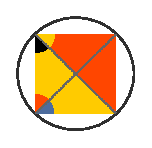
\includegraphics {figure.eps}}
     \caption{A one-column \{figure*\}[h!] after a section title.
      If text follows like below, it is easier to finish the section in
      \textbackslash onecolumn. If needed, you may revert to \textbackslash
      twocolumn when reaching the next page.}
      \label{fig5ap}
\end{figure*}


% If text follows like so 
\lipsum[1-2]
% it is easier to finish the page in onecolumn and revert to
% twocolumn when starting the next page if needed.}


\FloatBarrier %\usepackage{placeins}
\twocolumn
%____________________________________________________________
%       Wide floats at the start of an appendix: second method
%-------------------------------------------------------------
% To prevent a blank page, a second method is:
% - Declare the onecolumn float *
% - Declare the section under the float
% However, this method should be reserved to appendices
% containing only onecolumn tables or figures.
\begin{table*}[h!]
\section{Wide tables and figures after an appendix title: alternate method}
%

To prevent a blank page, a second method is to insert
the appendix title \underline{after} declaring the onecolumn float.
\newline This method should be reserved to appendices
containing only one-column floats\{figure*\} or \{table*\}
and no text.

\caption {A one-column \{table*\} \newline}
\label{table:2} 
\centering
\begin{tabular}{crrlcl}
\hline\hline             
ISO-L1551 & $F_{6.7}$~[mJy] & $\alpha_{6.7-14.3}$
& YSO type$^{d}$ & Status & Comments\\
\hline
  \multicolumn{6}{c}{\it New YSO candidates}\\ % To combine 6 columns into a single one
\hline
  1 & 1.56 $\pm$ 0.47 & --    & Class II$^{c}$ & New & Mid\\
  2 & 0.79:           & 0.97: & Class II ?     & New & \\
  3 & 4.95 $\pm$ 0.68 & 3.18  & Class II / III & New & \\
  5 & 1.44 $\pm$ 0.33 & 1.88  & Class II       & New & \\
  1 & 1.56 $\pm$ 0.47 & --    & Class II$^{c}$ & New & Mid\\
  2 & 0.79:           & 0.97: & Class II ?     & New & \\
  3 & 4.95 $\pm$ 0.68 & 3.18  & Class II / III & New & \\
  5 & 1.44 $\pm$ 0.33 & 1.88  & Class II       & New & \\
  1 & 1.56 $\pm$ 0.47 & --    & Class II$^{c}$ & New & Mid\\
  2 & 0.79:           & 0.97: & Class II ?     & New & \\
  3 & 4.95 $\pm$ 0.68 & 3.18  & Class II / III & New & \\
  5 & 1.44 $\pm$ 0.33 & 1.88  & Class II       & New & \\
  1 & 1.56 $\pm$ 0.47 & --    & Class II$^{c}$ & New & Mid\\
  2 & 0.79:           & 0.97: & Class II ?     & New & \\
  3 & 4.95 $\pm$ 0.68 & 3.18  & Class II / III & New & \\
  5 & 1.44 $\pm$ 0.33 & 1.88  & Class II       & New & \\

  2 & 0.79:           & 0.97: & Class II ?     & New & \\
  3 & 4.95 $\pm$ 0.68 & 3.18  & Class II / III & New & \\
  5 & 1.44 $\pm$ 0.33 & 1.88  & Class II       & New & \\
  1 & 1.56 $\pm$ 0.47 & --    & Class II$^{c}$ & New & Mid\\
  2 & 0.79:           & 0.97: & Class II ?     & New & \\
  3 & 4.95 $\pm$ 0.68 & 3.18  & Class II / III & New & \\
  5 & 1.44 $\pm$ 0.33 & 1.88  & Class II       & New & \\
  1 & 1.56 $\pm$ 0.47 & --    & Class II$^{c}$ & New & Mid\\
  2 & 0.79:           & 0.97: & Class II ?     & New & \\
  3 & 4.95 $\pm$ 0.68 & 3.18  & Class II / III & New & \\
  5 & 1.44 $\pm$ 0.33 & 1.88  & Class II       & New & \\
  1 & 1.56 $\pm$ 0.47 & --    & Class II$^{c}$ & New & Mid\\
  2 & 0.79:           & 0.97: & Class II ?     & New & \\
  3 & 4.95 $\pm$ 0.68 & 3.18  & Class II / III & New & \\
  5 & 1.44 $\pm$ 0.33 & 1.88  & Class II       & New & \\
\hline
  \multicolumn{6}{c}{\it Previously known YSOs} \\
\hline
  61 & 0.89 $\pm$ 0.58 & 1.77 & Class I & \object{HH 30} & Circumstellar disk\\
  96 & 38.34 $\pm$ 0.71 & 37.5& Class II& MHO 5          & Spectral type\\
\hline
\end{tabular}
\end{table*}


\FloatBarrier %\usepackage{placeins}
\twocolumn
%____________________________________________________________
% A long table in appendix
%------------------------------------------------------------
% This is the start of the page
\onecolumn
\section{Long tables in appendices}
For long tables (multipage) in appendices, we use the method described in appendix A.
For long landscape tables, please refer to Appendix E.
\begin{longtable}{lllrrr}
%

\caption{A long table}\\
\label{ltapp}

Catalogue& $M_{V}$ & Spectral & Distance & Mode & Count Rate \\
\hline
\endfirsthead
\caption{continued.}\\
\hline
Catalogue& $M_{V}$ & Spectral & Distance & Mode & Count Rate \\
\hline
\endhead
\hline
\endfoot
%%
Gl 33    & 6.37 & K2 V & 7.46 & S & 0.043170\\
Gl 66AB  & 6.26 & K2 V & 8.15 & S & 0.260478\\
Gl 68    & 5.87 & K1 V & 7.47 & P & 0.026610\\
         &      &      &      & H & 0.008686\\
Gl 86
\footnote{Source not included in the HRI catalog. See Sect.~5.4.2 for details.}
         & 5.92 & K0 V & 10.91& S & 0.058230\\
                  & 5.92 & K0 V & 10.91& S & 0.058230\\
Gl 33    & 6.37 & K2 V & 7.46 & S & 0.043170\\
Gl 66AB  & 6.26 & K2 V & 8.15 & S & 0.260478\\
Gl 68    & 5.87 & K1 V & 7.47 & P & 0.026610\\
         &      &      &      & H & 0.008686\\
Gl 86    & 5.92 & K0 V & 10.91& S & 0.058230\\            & 5.92 & K0 V & 10.91& S & 0.058230\\
Gl 33    & 6.37 & K2 V & 7.46 & S & 0.043170\\
Gl 66AB  & 6.26 & K2 V & 8.15 & S & 0.260478\\
Gl 68    & 5.87 & K1 V & 7.47 & P & 0.026610\\
         &      &      &      & H & 0.008686\\
Gl 86    & 5.92 & K0 V & 10.91& S & 0.058230\\            & 5.92 & K0 V & 10.91& S & 0.058230\\
Gl 33    & 6.37 & K2 V & 7.46 & S & 0.043170\\
Gl 66AB  & 6.26 & K2 V & 8.15 & S & 0.260478\\
Gl 68    & 5.87 & K1 V & 7.47 & P & 0.026610\\
         &      &      &      & H & 0.008686\\
Gl 86    & 5.92 & K0 V & 10.91& S & 0.058230\\            & 5.92 & K0 V & 10.91& S & 0.058230\\
Gl 33    & 6.37 & K2 V & 7.46 & S & 0.043170\\
Gl 66AB  & 6.26 & K2 V & 8.15 & S & 0.260478\\
Gl 68    & 5.87 & K1 V & 7.47 & P & 0.026610\\
         &      &      &      & H & 0.008686\\
Gl 86    & 5.92 & K0 V & 10.91& S & 0.058230\\            & 5.92 & K0 V & 10.91& S & 0.058230\\
Gl 33    & 6.37 & K2 V & 7.46 & S & 0.043170\\
Gl 66AB  & 6.26 & K2 V & 8.15 & S & 0.260478\\
Gl 68    & 5.87 & K1 V & 7.47 & P & 0.026610\\
         &      &      &      & H & 0.008686\\
Gl 86    & 5.92 & K0 V & 10.91& S & 0.058230\\            & 5.92 & K0 V & 10.91& S & 0.058230\\
Gl 33    & 6.37 & K2 V & 7.46 & S & 0.043170\\
Gl 66AB  & 6.26 & K2 V & 8.15 & S & 0.260478\\
Gl 68    & 5.87 & K1 V & 7.47 & P & 0.026610\\
         &      &      &      & H & 0.008686\\
Gl 86    & 5.92 & K0 V & 10.91& S & 0.058230\\            & 5.92 & K0 V & 10.91& S & 0.058230\\
Gl 33    & 6.37 & K2 V & 7.46 & S & 0.043170\\
Gl 66AB  & 6.26 & K2 V & 8.15 & S & 0.260478\\
Gl 68    & 5.87 & K1 V & 7.47 & P & 0.026610\\
         &      &      &      & H & 0.008686\\
Gl 86    & 5.92 & K0 V & 10.91& S & 0.058230\\            & 5.92 & K0 V & 10.91& S & 0.058230\\
Gl 33    & 6.37 & K2 V & 7.46 & S & 0.043170\\
Gl 66AB  & 6.26 & K2 V & 8.15 & S & 0.260478\\
Gl 68    & 5.87 & K1 V & 7.47 & P & 0.026610\\
         &      &      &      & H & 0.008686\\
Gl 86    & 5.92 & K0 V & 10.91& S & 0.058230\\            & 5.92 & K0 V & 10.91& S & 0.058230\\
Gl 33    & 6.37 & K2 V & 7.46 & S & 0.043170\\
Gl 66AB  & 6.26 & K2 V & 8.15 & S & 0.260478\\
Gl 68    & 5.87 & K1 V & 7.47 & P & 0.026610\\
         &      &      &      & H & 0.008686\\
Gl 86    & 5.92 & K0 V & 10.91& S & 0.058230\\
         & 5.92 & K0 V & 10.91& S & 0.058230\\
Gl 33    & 6.37 & K2 V & 7.46 & S & 0.043170\\
Gl 66AB  & 6.26 & K2 V & 8.15 & S & 0.260478\\
Gl 68    & 5.87 & K1 V & 7.47 & P & 0.026610\\
         &      &      &      & H & 0.008686\\
Gl 86    & 5.92 & K0 V & 10.91& S & 0.058230\\            & 5.92 & K0 V & 10.91& S & 0.058230\\
Gl 33    & 6.37 & K2 V & 7.46 & S & 0.043170\\
Gl 66AB  & 6.26 & K2 V & 8.15 & S & 0.260478\\
Gl 68    & 5.87 & K1 V & 7.47 & P & 0.026610\\
         &      &      &      & H & 0.008686\\
Gl 86    & 5.92 & K0 V & 10.91& S & 0.058230\\
         & 5.92 & K0 V & 10.91& S & 0.058230\\
Gl 33    & 6.37 & K2 V & 7.46 & S & 0.043170\\
Gl 66AB  & 6.26 & K2 V & 8.15 & S & 0.260478\\
Gl 68    & 5.87 & K1 V & 7.47 & P & 0.026610\\
         &      &      &      & H & 0.008686\\
Gl 86    & 5.92 & K0 V & 10.91& S & 0.058230\\            & 5.92 & K0 V & 10.91& S & 0.058230\\
Gl 33    & 6.37 & K2 V & 7.46 & S & 0.043170\\
Gl 66AB  & 6.26 & K2 V & 8.15 & S & 0.260478\\
Gl 68    & 5.87 & K1 V & 7.47 & P & 0.026610\\
         &      &      &      & H & 0.008686\\
Gl 86    & 5.92 & K0 V & 10.91& S & 0.058230\\            & 5.92 & K0 V & 10.91& S & 0.058230\\
Gl 33    & 6.37 & K2 V & 7.46 & S & 0.043170\\
Gl 66AB  & 6.26 & K2 V & 8.15 & S & 0.260478\\
Gl 68    & 5.87 & K1 V & 7.47 & P & 0.026610\\
         &      &      &      & H & 0.008686\\
Gl 86    & 5.92 & K0 V & 10.91& S & 0.058230\\            & 5.92 & K0 V & 10.91& S & 0.058230\\
Gl 33    & 6.37 & K2 V & 7.46 & S & 0.043170\\
Gl 66AB  & 6.26 & K2 V & 8.15 & S & 0.260478\\
Gl 68    & 5.87 & K1 V & 7.47 & P & 0.026610\\
         &      &      &      & H & 0.008686\\
Gl 86    & 5.92 & K0 V & 10.91& S & 0.058230\\   
\end{longtable}


\FloatBarrier %\usepackage{placeins}
\twocolumn
%_____________________________________________________________
% A rotated single page table
%-------------------------------------------------------------
% This is the start of the page
\begin{sidewaystable*}
\section{Rotated single page tables}
To prevent a blank page with \{sidewaystable*\}, we use the method
described in appendix B: declare the table first, and the section second.
%

\caption{A rotated table with \{sidewaystable*\}}
\label{table:4} 
\centering
\begin{tabular}{crrlcl}
\hline        
ISO-L1551 & $F_{6.7}$~[mJy] & $\alpha_{6.7-14.3}$ & YSO type$^{d}$ & Status & Comments \\
\hline
  \multicolumn{6}{c}{\it New YSO candidates}\\ % To combine 6 columns into a single one
\hline
  1 & 1.56 $\pm$ 0.47 & --    & Class II$^{c}$ & New & Mid\\
  2 & 0.79:           & 0.97: & Class II ?     & New & \\
  3 & 4.95 $\pm$ 0.68 & 3.18  & Class II / III & New & \\
  5 & 1.44 $\pm$ 0.33 & 1.88  & Class II       & New & \\
  1 & 1.56 $\pm$ 0.47 & --    & Class II$^{c}$ & New & Mid\\
  2 & 0.79:           & 0.97: & Class II ?     & New & \\
  3 & 4.95 $\pm$ 0.68 & 3.18  & Class II / III & New & \\
  5 & 1.44 $\pm$ 0.33 & 1.88  & Class II       & New & \\
  1 & 1.56 $\pm$ 0.47 & --    & Class II$^{c}$ & New & Mid\\
  2 & 0.79:           & 0.97: & Class II ?     & New & \\
  3 & 4.95 $\pm$ 0.68 & 3.18  & Class II / III & New & \\
  5 & 1.44 $\pm$ 0.33 & 1.88  & Class II       & New & \\
  1 & 1.56 $\pm$ 0.47 & --    & Class II$^{c}$ & New & Mid\\
  2 & 0.79:           & 0.97: & Class II ?     & New & \\
  3 & 4.95 $\pm$ 0.68 & 3.18  & Class II / III & New & \\
  5 & 1.44 $\pm$ 0.33 & 1.88  & Class II       & New & \\
  1 & 1.56 $\pm$ 0.47 & --    & Class II$^{c}$ & New & Mid\\
  2 & 0.79:           & 0.97: & Class II ?     & New & \\
  3 & 4.95 $\pm$ 0.68 & 3.18  & Class II / III & New & \\
  5 & 1.44 $\pm$ 0.33 & 1.88  & Class II       & New & \\
  1 & 1.56 $\pm$ 0.47 & --    & Class II$^{c}$ & New & Mid\\
  2 & 0.79:           & 0.97: & Class II ?     & New & \\
  3 & 4.95 $\pm$ 0.68 & 3.18  & Class II / III & New & \\
  5 & 1.44 $\pm$ 0.33 & 1.88  & Class II       & New & \\
  1 & 1.56 $\pm$ 0.47 & --    & Class II$^{c}$ & New & Mid\\
  2 & 0.79:           & 0.97: & Class II ?     & New & \\
  3 & 4.95 $\pm$ 0.68 & 3.18  & Class II / III & New & \\
  5 & 1.44 $\pm$ 0.33 & 1.88  & Class II       & New & \\
\hline
  \multicolumn{6}{c}{\it Previously known YSOs} \\
\hline
  61 & 0.89 $\pm$ 0.58 & 1.77 & Class I & \object{HH 30} & Circumstellar disk\\
  96 & 38.34 $\pm$ 0.71 & 37.5& Class II& MHO 5          & Spectral type\\
\hline
\end{tabular}
\end{sidewaystable*}


\FloatBarrier %\usepackage{placeins}
\twocolumn
%_____________________________________________________________
% A rotated long table in appendix
%-------------------------------------------------------------
% This is the start of the page
\onecolumn
\begin{landscape}
\section{Rotated long tables in appendices}
For rotated long tables in appendices, we use the method
described in appendix A, combined with \{landscape\}.
\begin{longtable}{lllrrr}
%

\caption{A long landscape table}\\
\label{lsltapp} 

Catalogue& $M_{V}$ & Spectral & Distance & Mode & Count Rate \\
\hline
\endfirsthead
\caption{continued.}\\
\hline\hline
Catalogue& $M_{V}$ & Spectral & Distance & Mode & Count Rate \\
\hline
\endhead
\hline
\endfoot
%%
Gl 33    & 6.37 & K2 V & 7.46 & S & 0.043170\\
Gl 66AB  & 6.26 & K2 V & 8.15 & S & 0.260478\\
Gl 68    & 5.87 & K1 V & 7.47 & P & 0.026610\\
         &      &      &      & H & 0.008686\\
Gl 86
\footnote{Source not included in the HRI catalog. See Sect.~5.4.2 for details.}
         & 5.92 & K0 V & 10.91& S & 0.058230\\
         Gl 33    & 6.37 & K2 V & 7.46 & S & 0.043170\\
Gl 66AB  & 6.26 & K2 V & 8.15 & S & 0.260478\\
Gl 68    & 5.87 & K1 V & 7.47 & P & 0.026610\\
         &      &      &      & H & 0.008686\\
Gl 86    & 5.92 & K0 V & 10.91& S & 0.058230\\
Gl 33    & 6.37 & K2 V & 7.46 & S & 0.043170\\
Gl 66AB  & 6.26 & K2 V & 8.15 & S & 0.260478\\
Gl 68    & 5.87 & K1 V & 7.47 & P & 0.026610\\
         &      &      &      & H & 0.008686\\
Gl 86    & 5.92 & K0 V & 10.91& S & 0.058230\\   Gl 33    & 6.37 & K2 V & 7.46 & S & 0.043170\\
Gl 66AB  & 6.26 & K2 V & 8.15 & S & 0.260478\\
Gl 68    & 5.87 & K1 V & 7.47 & P & 0.026610\\
         &      &      &      & H & 0.008686\\
Gl 86    & 5.92 & K0 V & 10.91& S & 0.058230\\   Gl 33    & 6.37 & K2 V & 7.46 & S & 0.043170\\
Gl 66AB  & 6.26 & K2 V & 8.15 & S & 0.260478\\
Gl 68    & 5.87 & K1 V & 7.47 & P & 0.026610\\
         &      &      &      & H & 0.008686\\
Gl 86    & 5.92 & K0 V & 10.91& S & 0.058230\\   Gl 33    & 6.37 & K2 V & 7.46 & S & 0.043170\\
Gl 66AB  & 6.26 & K2 V & 8.15 & S & 0.260478\\
Gl 68    & 5.87 & K1 V & 7.47 & P & 0.026610\\
         &      &      &      & H & 0.008686\\
Gl 86    & 5.92 & K0 V & 10.91& S & 0.058230\\   Gl 33    & 6.37 & K2 V & 7.46 & S & 0.043170\\
Gl 66AB  & 6.26 & K2 V & 8.15 & S & 0.260478\\
Gl 68    & 5.87 & K1 V & 7.47 & P & 0.026610\\
         &      &      &      & H & 0.008686\\
Gl 86    & 5.92 & K0 V & 10.91& S & 0.058230\\   Gl 33    & 6.37 & K2 V & 7.46 & S & 0.043170\\
Gl 66AB  & 6.26 & K2 V & 8.15 & S & 0.260478\\
Gl 68    & 5.87 & K1 V & 7.47 & P & 0.026610\\
         &      &      &      & H & 0.008686\\
Gl 86    & 5.92 & K0 V & 10.91& S & 0.058230\\   Gl 33    & 6.37 & K2 V & 7.46 & S & 0.043170\\
Gl 66AB  & 6.26 & K2 V & 8.15 & S & 0.260478\\
Gl 68    & 5.87 & K1 V & 7.47 & P & 0.026610\\
         &      &      &      & H & 0.008686\\
Gl 86    & 5.92 & K0 V & 10.91& S & 0.058230\\   Gl 33    & 6.37 & K2 V & 7.46 & S & 0.043170\\
Gl 66AB  & 6.26 & K2 V & 8.15 & S & 0.260478\\
Gl 68    & 5.87 & K1 V & 7.47 & P & 0.026610\\
         &      &      &      & H & 0.008686\\
Gl 86    & 5.92 & K0 V & 10.91& S & 0.058230\\   Gl 33    & 6.37 & K2 V & 7.46 & S & 0.043170\\
Gl 66AB  & 6.26 & K2 V & 8.15 & S & 0.260478\\
Gl 68    & 5.87 & K1 V & 7.47 & P & 0.026610\\
         &      &      &      & H & 0.008686\\
Gl 86    & 5.92 & K0 V & 10.91& S & 0.058230\\   Gl 33    & 6.37 & K2 V & 7.46 & S & 0.043170\\
Gl 66AB  & 6.26 & K2 V & 8.15 & S & 0.260478\\
Gl 68    & 5.87 & K1 V & 7.47 & P & 0.026610\\
         &      &      &      & H & 0.008686\\
Gl 86    & 5.92 & K0 V & 10.91& S & 0.058230\\   Gl 33    & 6.37 & K2 V & 7.46 & S & 0.043170\\
Gl 66AB  & 6.26 & K2 V & 8.15 & S & 0.260478\\
Gl 68    & 5.87 & K1 V & 7.47 & P & 0.026610\\
         &      &      &      & H & 0.008686\\
Gl 86    & 5.92 & K0 V & 10.91& S & 0.058230\\   Gl 33    & 6.37 & K2 V & 7.46 & S & 0.043170\\
Gl 66AB  & 6.26 & K2 V & 8.15 & S & 0.260478\\
Gl 68    & 5.87 & K1 V & 7.47 & P & 0.026610\\
         &      &      &      & H & 0.008686\\
Gl 86    & 5.92 & K0 V & 10.91& S & 0.058230\\   
\end{longtable}
\end{landscape}


\FloatBarrier %\usepackage{placeins}
\clearpage


\end{appendix}
\end{document}